% !TEX root = ps3_text.tex

\documentclass[12pt]{article}

% Geometry
\usepackage[a4paper, left=3cm, right=2.5cm, top=2.5cm, bottom=3cm]{geometry}

% Font encoding
\usepackage[utf8]{inputenc} % UTF-8 encoding
\usepackage[T1]{fontenc} % Font encoding
\usepackage{times}

% Math packages
\usepackage{amsmath} % Basic math symbols and environments
\usepackage{amssymb} % Additional math symbols
\usepackage{amsfonts} % Math fonts

% Text packages
\usepackage{parskip}
\setlength{\parskip}{1em}
\usepackage{hyperref}
\hypersetup{
    colorlinks=true,
    linkcolor=blue,
}

% Pictures
\usepackage{graphicx}
\usepackage{float}

% Lists
\usepackage{enumitem}
\setlist[itemize]{itemsep = -0.5em, topsep = -0.5em}

% Bibliography
%\usepackage{cite}

% Loops:
\usepackage{pgffor}

% Extra commands:
\makeatletter
\renewcommand{\maketitle}{
  \begin{center}
    {\Huge \@title}\\[2em]
    {\large \@author \hfill \@date}\\[2em]
  \end{center}
}
\makeatother


% Title and author
\title{Econometrics II - Problem Set 3}
\author{Ricardo Semião e Castro}
\date{05/2024}


\begin{document}

\maketitle

\section*{Exploratory Data Analysis}

This section is dedicated to the exploratory analysis made for questions 1. and 4.

We can see the time series values below. Exchange had a clear trend, so it was detrended using a HPfilter with $\lambda = 100$ for yearly data.

\begin{figure}[H]
    \centering
    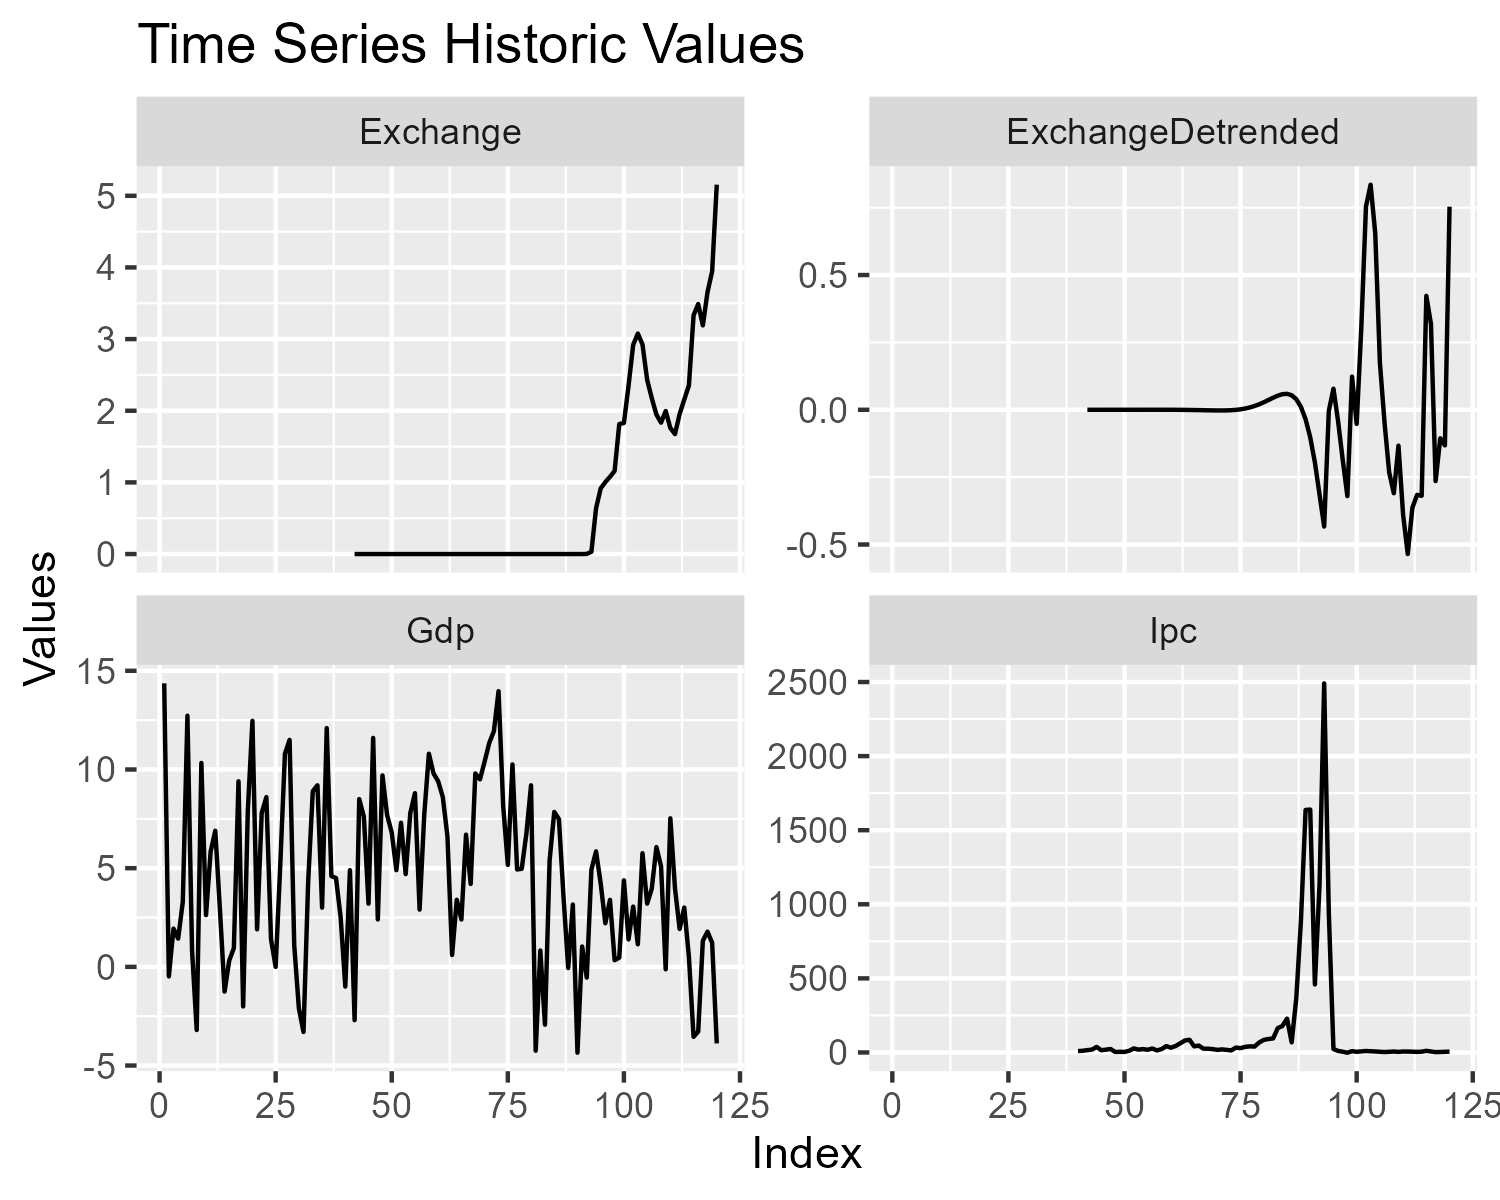
\includegraphics[width=0.8\textwidth]{figures/explore_values.png}
\end{figure}

It is also interesting to consider the plots of the ACF of the series.

\begin{figure}[H]
    \centering
    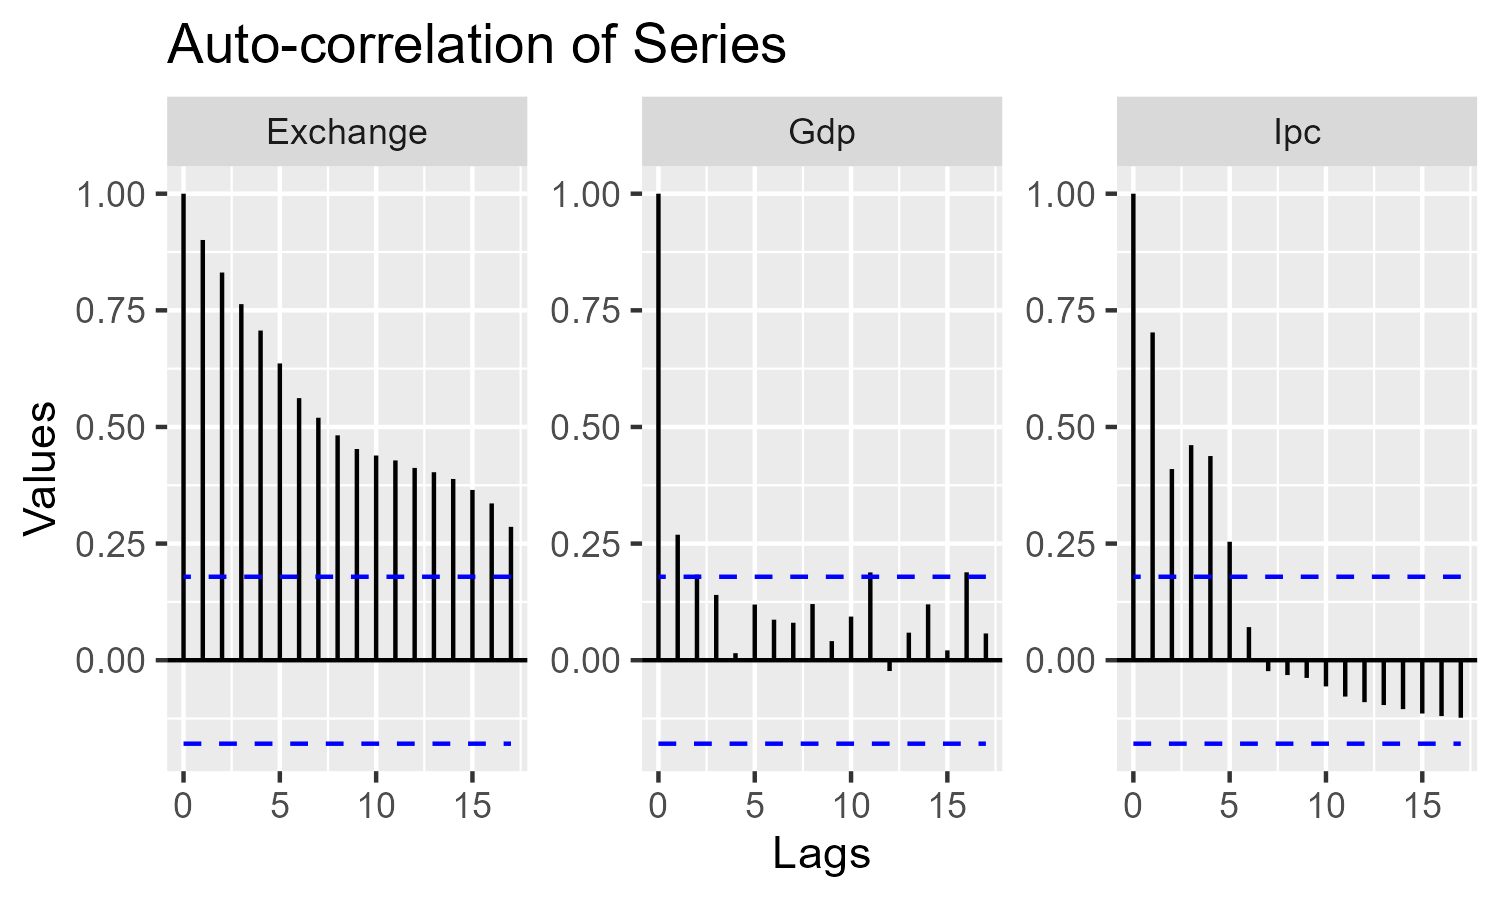
\includegraphics[width=0.8\textwidth]{figures/explore_acf.png}
\end{figure}

We can see that Exchange presents a trend, and strong memory. With this motivation, I ran the ADF test for the series. The results can be seen below.


\begin{table}[!htbp] \centering 
  \caption{} 
  \label{tb:dftest_exchange} 
\begin{tabular}{@{\extracolsep{5pt}} cccc} 
\\[-1.8ex]\hline 
\hline \\[-1.8ex] 
Lag & Type 1 & Type 2 & Type 3 \\ 
\hline \\[-1.8ex] 
0 & 3.8
(0.99) & 2.9
(0.99) & 0.82
(0.99) \\ 
1 & 2.53
(0.99) & 1.93
(0.99) & 0.21
(0.99) \\ 
2 & 2.28
(0.99) & 1.73
(0.99) & 0.07
(0.99) \\ 
\hline \\[-1.8ex] 
\end{tabular} 
\end{table} 


\begin{table}[!htbp] \centering 
  \caption{} 
  \label{tb:dftest_gdp} 
\begin{tabular}{@{\extracolsep{5pt}} cccc} 
\\[-1.8ex]\hline 
\hline \\[-1.8ex] 
Lag & Type 1 & Type 2 & Type 3 \\ 
\hline \\[-1.8ex] 
0 & -5.25
(0.01) & -8.18
(0.01) & -8.32
(0.01) \\ 
1 & -3.21
(0.01) & -5.46
(0.01) & -5.67
(0.01) \\ 
2 & -2.46
(0.02) & -4.41
(0.01) & -4.65
(0.01) \\ 
\hline \\[-1.8ex] 
\end{tabular} 
\end{table} 


\begin{table}[!htbp] \centering 
  \caption{ADF Test - IPC} 
  \label{tb:dftest_ipc} 
\begin{tabular}{@{\extracolsep{5pt}} cccc} 
\\[-1.8ex]\hline 
\hline \\[-1.8ex] 
Lag & Type 1 & Type 2 & Type 3 \\ 
\hline \\[-1.8ex] 
0 & -3.45
(0.01) & -3.68
(0.01) & -3.67
(0.03) \\ 
1 & -3.67
(0.01) & -3.97
(0.01) & -3.96
(0.02) \\ 
2 & -1.91
(0.06) & -2.07
(0.3) & -2.03
(0.56) \\ 
\hline \\[-1.8ex] 
\end{tabular} 
\end{table} 


Table 1 indicates that the series Exchange  probably is non-stationary, while the other two are stationary. So, it was probably more suited to do a differencing, instead of a detrending. For simplicity, the variable was included with trend in the models.



\section*{Question 1}

The results can be seen below. The row 'predictions' and 'MSE' are related to the prediction for 2020.


\begin{table}[H] \centering 
  \caption{} 
  \label{tb:ardl} 
\begin{tabular}{@{\extracolsep{5pt}}lcccc} 
\\[-1.8ex]\hline 
\hline \\[-1.8ex] 
 & \multicolumn{4}{c}{\textit{Dependent variable:}} \\ 
\cline{2-5} 
\\[-1.8ex] & \multicolumn{4}{c}{GDP Growth} \\ 
\\[-1.8ex] & (1) & (2) & (3) & (4)\\ 
\hline \\[-1.8ex] 
 lag(Gdp, 1) & 0.323$^{***}$ & 0.368$^{***}$ & 0.282$^{**}$ & 0.373$^{***}$ \\ 
  & (0.114) & (0.111) & (0.121) & (0.109) \\ 
  lag(Gdp, 2) & 0.230$^{**}$ & 0.264$^{**}$ & 0.195$^{*}$ & 0.273$^{**}$ \\ 
  & (0.110) & (0.110) & (0.117) & (0.107) \\ 
  lag(Exchange, 1) & $-$0.591 &  & $-$1.497 &  \\ 
  & (0.401) &  & (2.051) &  \\ 
  lag(Exchange, 2) &  &  & 0.751 &  \\ 
  &  &  & (2.122) &  \\ 
  lag(Ipc, 1) &  & 0.0003 & $-$0.0004 &  \\ 
  &  & (0.001) & (0.001) &  \\ 
  lag(Ipc, 2) &  & $-$0.001 & $-$0.001 &  \\ 
  &  & (0.001) & (0.001) &  \\ 
  Constant & 2.490$^{***}$ & 1.777$^{**}$ & 3.200$^{***}$ & 1.625$^{**}$ \\ 
  & (0.883) & (0.746) & (1.085) & (0.665) \\ 
 \hline \\[-1.8ex] 
Predictions & 0.96 & 2.7 & 0.72 & 2.57 \\ 
MSE & 23.43 & 43.24 & 21.19 & 41.55 \\ 
Observations & 76 & 76 & 76 & 76 \\ 
R$^{2}$ & 0.333 & 0.318 & 0.349 & 0.313 \\ 
Adjusted R$^{2}$ & 0.305 & 0.279 & 0.292 & 0.294 \\ 
Residual Std. Error & 3.382 (df = 72) & 3.444 (df = 71) & 3.414 (df = 69) & 3.409 (df = 73) \\ 
\hline 
\hline \\[-1.8ex] 
\textit{Note:}  & \multicolumn{4}{r}{$^{*}$p$<$0.1; $^{**}$p$<$0.05; $^{***}$p$<$0.01} \\ 
\end{tabular} 
\end{table} 


Via the MSE, we can see that the model generates the best prediction is from model 3. This makes sense, given that it is the most complex model, while seeming to be not too complex, not suffering from overfitting.



\section*{Question 2}

Let $\phi_j$ denote the vector of coefficients of each lag $j$ in the $VAR(p)$ model, and $\epsilon_t$ the error term. Then, we can write the model and take the expectancy of both sides:

$$
E[Y_t] = c + \phi_1E[Y_{t-1}] + \dots + \phi_pE[Y_{t-p}] + E[\epsilon_t]
$$

As $\{Y_t\}$ is covariance-stationary, $E[Y_{t}] = E[Y_{t-1}] = \dots = E[Y_{t-p}]$ Denote this value by $\mu$. Also $E[\epsilon_t] = 0$. So, we have:

\begin{align*}
    &\mu = c + \phi_1\mu + \dots + \phi_p\mu\\
    &(I - \phi_1 - \dots - \phi_p)\mu = c\\
    &\mu = (I - \phi_1 - \dots - \phi_p)^{-1}c
\end{align*}




\section*{Question 3}

First, note that $\Gamma_{-j} = E[(Y_t - \mu)(Y_{t+j} - \mu)']$.

Then:

\begin{align*}
    \Gamma'_j &= E[(Y_{t-j} - \mu)(Y_t - \mu)']\\
    &= E[(Y_{t-j + j} - \mu)(Y_{t + j} - \mu)']\\
    &= \Gamma_{-j}
\end{align*}

The second line step came from ${Y_t}$ being covariance-stationary, "the window doesn't matter", i.e.:

$$
E[(Y_{t-j + k} - \mu)(Y_{t + k} - \mu)'] = E[(Y_{t-j} - \mu)(Y_{t} - \mu)'],~~ \forall k \in \mathbb{N}
$$



\section*{Question 6}

\subsection*{Item 1.}

The results, for each model, can be seen below. I used the detrended version of Exchange.


\begin{table}[H] \centering 
  \caption{VAR(1)} 
  \label{tb:var_1} 
\begin{tabular}{@{\extracolsep{5pt}}lccc} 
\\[-1.8ex]\hline 
\hline \\[-1.8ex] 
 & \multicolumn{3}{c}{\textit{Dependent variable:}} \\ 
\cline{2-4} 
 & Gdp & Ipc & ExchangeDetrended \\ 
\hline \\[-1.8ex] 
 Gdp.l1 & 0.445$^{***}$ & $-$10.312 & 0.002 \\ 
  & (0.104) & (8.593) & (0.005) \\ 
  Ipc.l1 & $-$0.001 & 0.672$^{***}$ & 0.00002 \\ 
  & (0.001) & (0.087) & (0.00005) \\ 
  ExchangeDetrended.l1 & 1.016 & $-$77.375 & 0.698$^{***}$ \\ 
  & (1.967) & (162.533) & (0.088) \\ 
  const & 2.787$^{***}$ & 97.979$^{*}$ & $-$0.016 \\ 
  & (0.687) & (56.757) & (0.031) \\ 
 \hline \\[-1.8ex] 
Predictions & 3.19 & 98.58 & -0.11 \\ 
MSE & 50.01 & 8641.3 & 0.74 \\ 
Observations & 77 & 77 & 77 \\ 
R$^{2}$ & 0.227 & 0.504 & 0.474 \\ 
Adjusted R$^{2}$ & 0.196 & 0.483 & 0.452 \\ 
Residual Std. Error (df = 73) & 3.635 & 300.352 & 0.162 \\ 
\hline 
\hline \\[-1.8ex] 
\textit{Note:}  & \multicolumn{3}{r}{$^{*}$p$<$0.1; $^{**}$p$<$0.05; $^{***}$p$<$0.01} \\ 
\end{tabular} 
\end{table} 


\begin{table}[H] \centering 
  \caption{VAR(2)} 
  \label{tb:var_2} 
\begin{tabular}{@{\extracolsep{5pt}}lccc} 
\\[-1.8ex]\hline 
\hline \\[-1.8ex] 
 & \multicolumn{3}{c}{\textit{Dependent variable:}} \\ 
\cline{2-4} 
 & Gdp & Ipc & Exchange \\ 
\hline \\[-1.8ex] 
 Gdp.l1 & 0.282$^{**}$ & $-$18.671$^{*}$ & 0.001 \\ 
  & (0.121) & (10.306) & (0.007) \\ 
  Ipc.l1 & $-$0.0004 & 0.707$^{***}$ & 0.0001$^{*}$ \\ 
  & (0.001) & (0.120) & (0.0001) \\ 
  Exchange.l1 & $-$1.497 & $-$194.682 & 1.334$^{***}$ \\ 
  & (2.051) & (175.155) & (0.121) \\ 
  Gdp.l2 & 0.195$^{*}$ & $-$13.218 & $-$0.0002 \\ 
  & (0.117) & (9.982) & (0.007) \\ 
  Ipc.l2 & $-$0.001 & $-$0.173 & $-$0.00005 \\ 
  & (0.001) & (0.117) & (0.0001) \\ 
  Exchange.l2 & 0.751 & 112.603 & $-$0.309$^{**}$ \\ 
  & (2.122) & (181.280) & (0.125) \\ 
  const & 3.200$^{***}$ & 288.045$^{***}$ & 0.0001 \\ 
  & (1.085) & (92.642) & (0.064) \\ 
 \hline \\[-1.8ex] 
Predictions & 0.72 & -112.25 & 4.13 \\ 
MSE & 21.19 & 13893.94 & 1.04 \\ 
Observations & 76 & 76 & 76 \\ 
R$^{2}$ & 0.349 & 0.557 & 0.973 \\ 
Adjusted R$^{2}$ & 0.292 & 0.519 & 0.971 \\ 
Residual Std. Error (df = 69) & 3.414 & 291.590 & 0.201 \\ 
\hline 
\hline \\[-1.8ex] 
\textit{Note:}  & \multicolumn{3}{r}{$^{*}$p$<$0.1; $^{**}$p$<$0.05; $^{***}$p$<$0.01} \\ 
\end{tabular} 
\end{table} 


\begin{table}[H] \centering 
  \caption{VAR(3)} 
  \label{tb:var_3} 
\begin{tabular}{@{\extracolsep{5pt}}lccc} 
\\[-1.8ex]\hline 
\hline \\[-1.8ex] 
 & \multicolumn{3}{c}{\textit{Dependent variable:}} \\ 
\cline{2-4} 
 & Gdp & Ipc & ExchangeDetrended \\ 
\hline \\[-1.8ex] 
 Gdp.l1 & 0.332$^{**}$ & $-$6.670 & 0.004 \\ 
  & (0.126) & (9.532) & (0.006) \\ 
  Ipc.l1 & 0.0004 & 0.874$^{***}$ & 0.0001 \\ 
  & (0.001) & (0.110) & (0.0001) \\ 
  ExchangeDetrended.l1 & 0.470 & 3.501 & 0.866$^{***}$ \\ 
  & (2.806) & (212.551) & (0.125) \\ 
  Gdp.l2 & 0.303$^{**}$ & $-$8.556 & 0.004 \\ 
  & (0.126) & (9.542) & (0.006) \\ 
  Ipc.l2 & $-$0.001 & $-$0.568$^{***}$ & $-$0.00000 \\ 
  & (0.002) & (0.141) & (0.0001) \\ 
  ExchangeDetrended.l2 & 0.779 & $-$170.812 & $-$0.203 \\ 
  & (3.642) & (275.915) & (0.163) \\ 
  Gdp.l3 & 0.022 & 8.080 & $-$0.008 \\ 
  & (0.120) & (9.123) & (0.005) \\ 
  Ipc.l3 & 0.00002 & 0.515$^{***}$ & $-$0.0001 \\ 
  & (0.001) & (0.111) & (0.0001) \\ 
  ExchangeDetrended.l3 & 0.748 & 277.678 & $-$0.090 \\ 
  & (2.814) & (213.148) & (0.126) \\ 
  const & 1.567$^{*}$ & 61.938 & 0.005 \\ 
  & (0.842) & (63.799) & (0.038) \\ 
 \hline \\[-1.8ex] 
Predictions & 2.2 & -3.31 & -0.06 \\ 
MSE & 36.94 & 79.79 & 0.67 \\ 
Observations & 75 & 75 & 75 \\ 
R$^{2}$ & 0.332 & 0.645 & 0.552 \\ 
Adjusted R$^{2}$ & 0.239 & 0.596 & 0.490 \\ 
Residual Std. Error (df = 65) & 3.550 & 268.921 & 0.159 \\ 
\hline 
\hline \\[-1.8ex] 
\textit{Note:}  & \multicolumn{3}{r}{$^{*}$p$<$0.1; $^{**}$p$<$0.05; $^{***}$p$<$0.01} \\ 
\end{tabular} 
\end{table} 


Comparing the predictions, $VAR(1)$ yielded $0.23$ (MSE of $16.92$), $VAR(2)$ yielded $0.72$ (MSE of $21.19$), and $VAR(3)$ yielded $0.8$ (MSE of $21.88$). $VAR(1)$ was the best.

For yearly data, we don't normally need to use too many lags to capture the dynamic of the problem, specially when using multiple series. This might be why $VAR(1)$ had the better prevision.


\subsection*{Item 2.}

The chosen order was (Ipc, Gdp, Exchange). The choice lies in the analysis of the level of rigidity of each variable. We have lots of empirical evidence to consider price rigidities, such that GDP should respond to IPC. The inflation could be set by the BC given the GDP, or react to the state of the economy, but this shouldn't be too intense, and one could argue relatively exogenous shocks on inflation. Lastly, the exchange rate should be the most endogenous variable, as the value of the currency is set by expectations, which relate to both GDP and IPC, and propagate quickly, given the high liquidity of the exchange market.

The IRFs with the Cholesky decomposition in the order above can be seen below.

\begin{figure}[H]
    \centering
    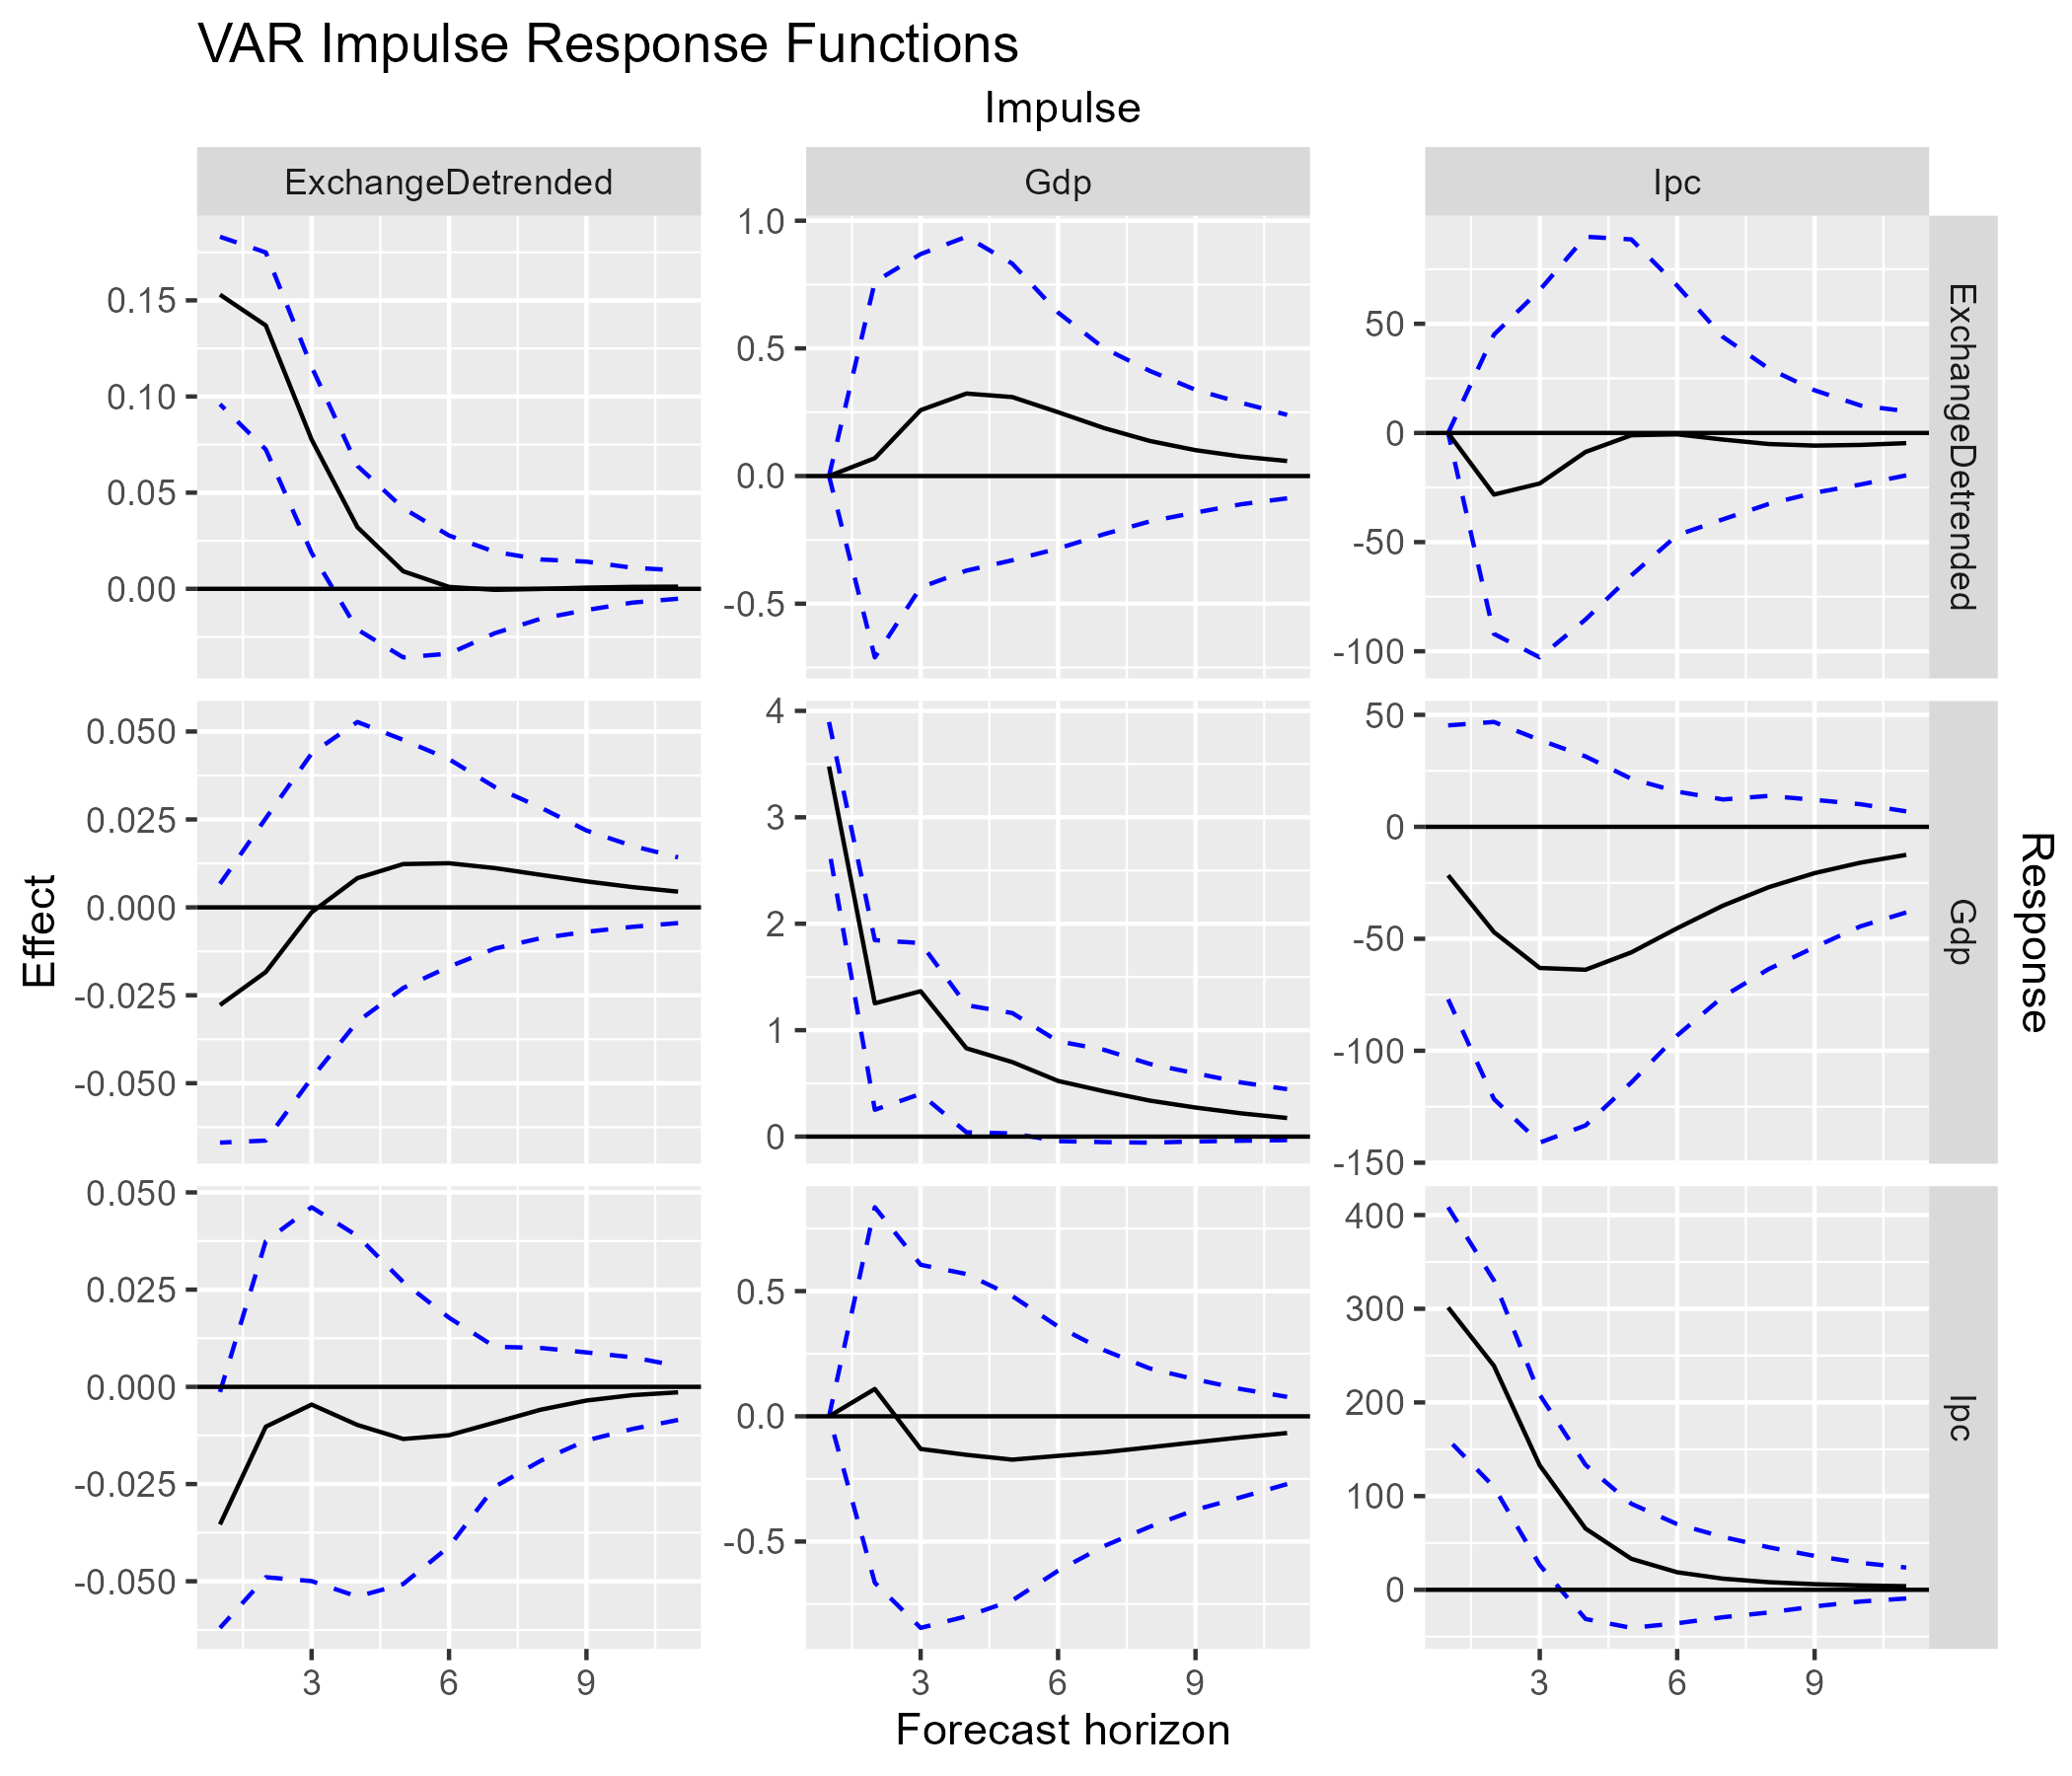
\includegraphics[width=0.8\textwidth]{figures/irfs.png}
\end{figure}

The results are not really credible. We have no statistically significant response of GDP given a shock of inflation, which contradicts our assumption of price rigidities. The exchange rate also doesn't present significant responses to IPC and GDP.

These poor results are not surprising, given the low quality of the data and the decomposition assumptions. For the data, there have been many structural breaks in Brazil's economy since 1949, as the exploratory analysis showed. There have been the military dictatorship, hyperinflation, "the economic miracle" the Real plan, etc. All of this makes a fixed-coefficient VAR very unreliable.

As for the assumptions, as stated before, are very ambiguous, and there are ways to justify IPC also responding to GDP via BC's choice and other market mechanisms. Also, not always the exchange market is so liquid.


\end{document}
